\section{Event simulation}

Simulated events, also known as Monte Carlo (MC) events, are crucial when 
designing and conducting a search. Prior to the analysis of the LHC data 
both simulated signal and Standard Model background events
are typically used to design the event reconstruction, determine the optimal 
event selection, estimate the signal efficiency and the background rate.

When generating the simulated events, partons from distribution functions 
(CTEQ \cite{Bourilkov:2006cj}) undergo hard scattering in \PYTHIA \cite{PYTHIA}. 
The parton showers are then hadronized again with \PYTHIA and the unstable particles are decayed.
The particles outgoing from the collision point are then propagated through the CMS detector 
using GEANT4 \cite{GEANT4} which provides a full description of the detector geometry
and simulates
the interactions of particles with the detector material. The energy deposits are digitized
to emulate the response of the detector electronics followed by event reconstruction,
as for data. Additionally, in order to reproduce the 
condition of multiple simultaneous interactions occurring in the same crossing of the 
bunches, a number of simulated hard-scattering events are overlaid on top of the primary 
simulated event. The distribution of the number of simultaneous interactions overlaid in the
MC data samples is chosen such that it approximates the LHC running conditions.

For the purpose of the search signal MC simulation samples are generated to
simulate non-SM Higgs (\Higgs) production through gluon fusion ($gg \to \Higgs$). 
Subsequently the \Higgs~is forced to decay to two long-lived, spin~0, exotic particles
($\Higgs \to 2\X$), which each then decays to quark-antiquark pairs ($\X \to \qq$).
The long-lived exotic \X decays to any flavor $\qq$ pair, excluding \ttbar, with equal probability. Samples
with different combinations of \Higgs~masses ($M_{\Higgs}$ = 120, 200, 400, 1000 \GeV ) and \X~boson masses
($M_{\X}$ = 20, 50, 150, 350 \GeV) are generated. These are listed in Table~\ref{tab:signalMC}.

\begin{table}[hbtp]
\begin{center}
\begin{tabular}{ccc}
\hline
  $M_{\Higgs}$ (\GeV) & $M_{\X}$ (\GeV) & $c\tau$ (cm) \\
\hline
       1000      &       350      &     3.5, 35, 350      \\
       1000      &       150      &     1, 10, 100      \\
       1000      &        50      &     0.4, 4, 40      \\
       1000      &        20      &     0.15, 1.5, 15       \\
       ~400      &       150      &     4, 40, 400      \\
       ~400      &        50      &     0.8, 8, 80      \\
       ~400      &        20      &     0.4, 4, 40      \\
       ~200      &        50      &     2, 20, 200      \\
       ~200      &        20      &     0.7, 7, 70      \\
       ~120      &        50      &     5, 50, 500      \\
       ~120      &        20      &     1.3, 13, 130      \\
\hline
\end{tabular}
\caption{Simulated signal samples used in the analysis. The masses of the \Higgs and \X bosons are given,
as is the mean proper decay length of the \X~boson. \label{tab:signalMC}}
\end{center}
\end{table}

 The
\X boson ~lifetime used in these samples is chosen to give a mean transverse decay length of approximately
3\cm, 30\cm and 300\cm in the laboratory frame. Such a selection of laboratory frame lifetimes is chosen in
order to maximally explore the capabilities of the CMS detector for reconstructing long-lived particles.
The distributions of the simulated \Higgs transverse momentum, $p_T$, and resulting \X $p_T$ and 
pseudorapidity, $\eta$, spectra for selected signal
models are presented in Figure \ref{fig:sigHX}.

\begin{figure}[htbp]
\centering
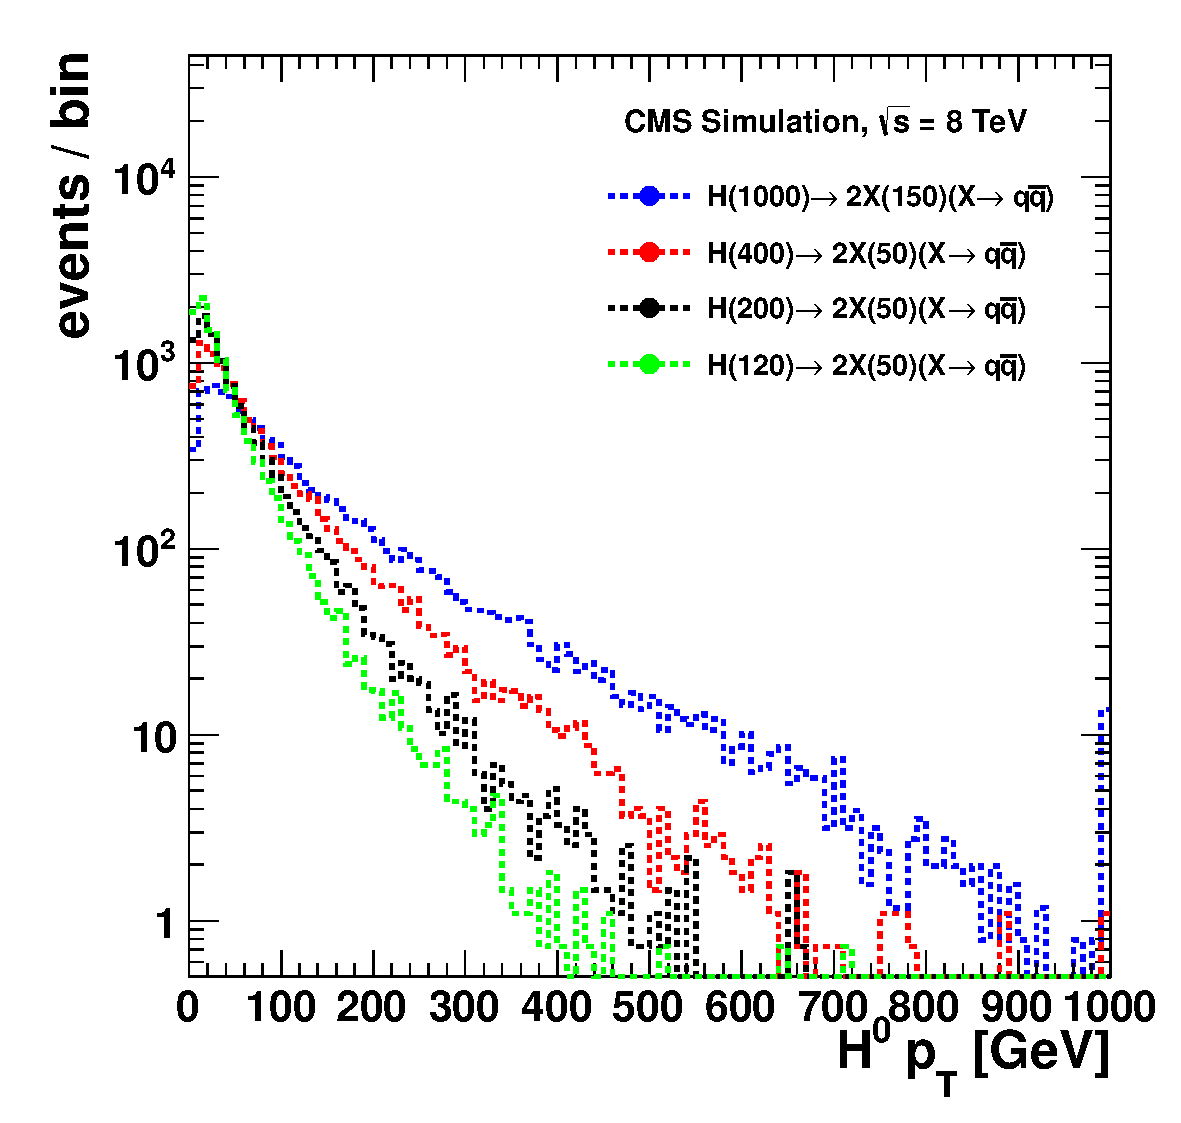
\includegraphics[width=0.495\textwidth]{plots/signal/hpt.pdf}
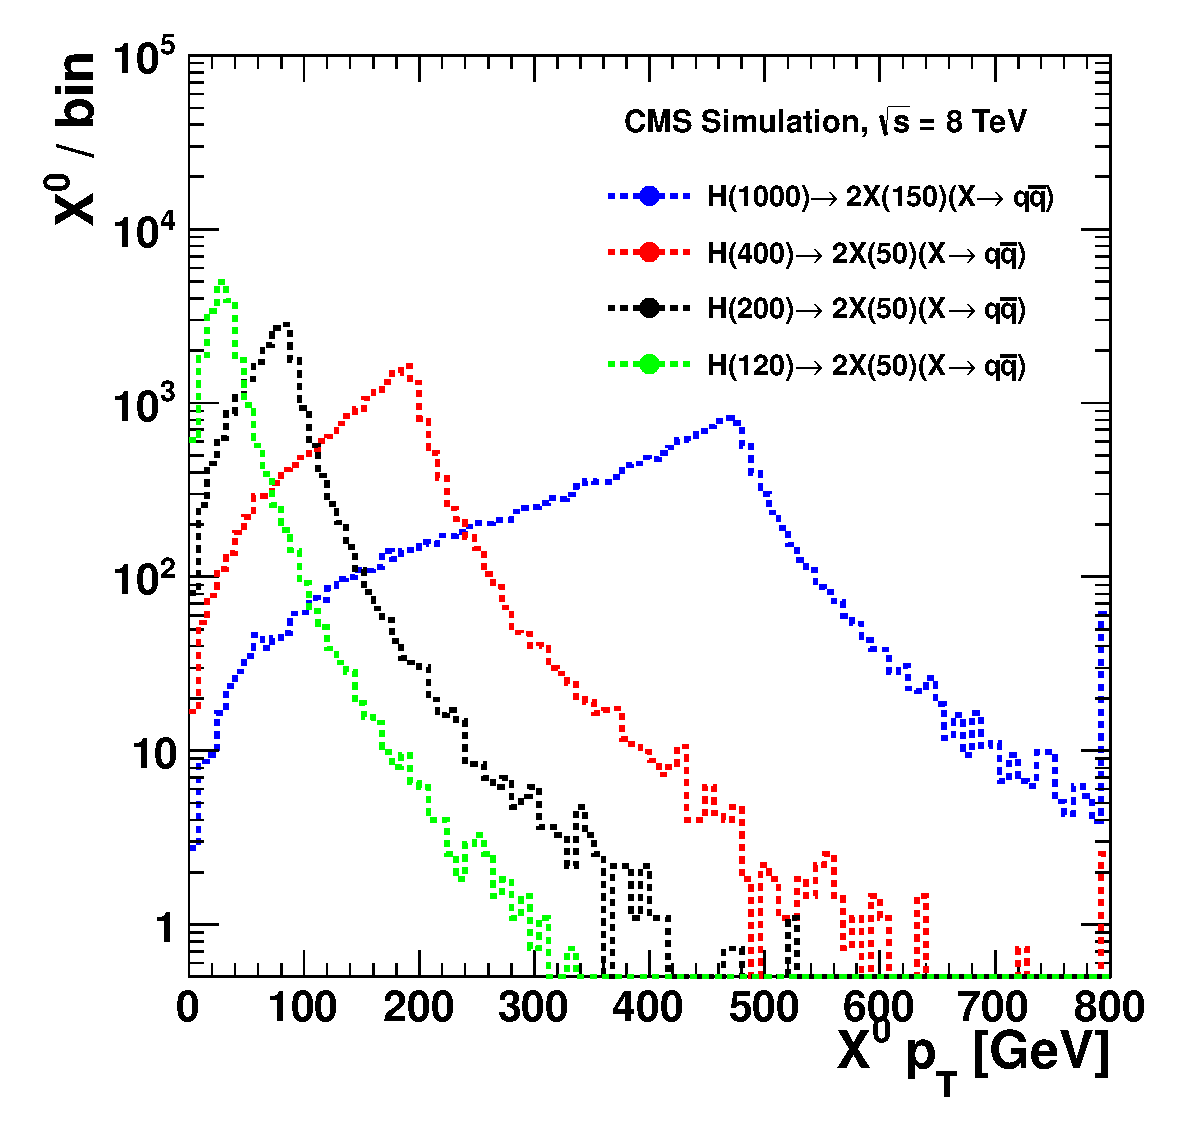
\includegraphics[width=0.495\textwidth]{plots/signal/xpt.pdf}
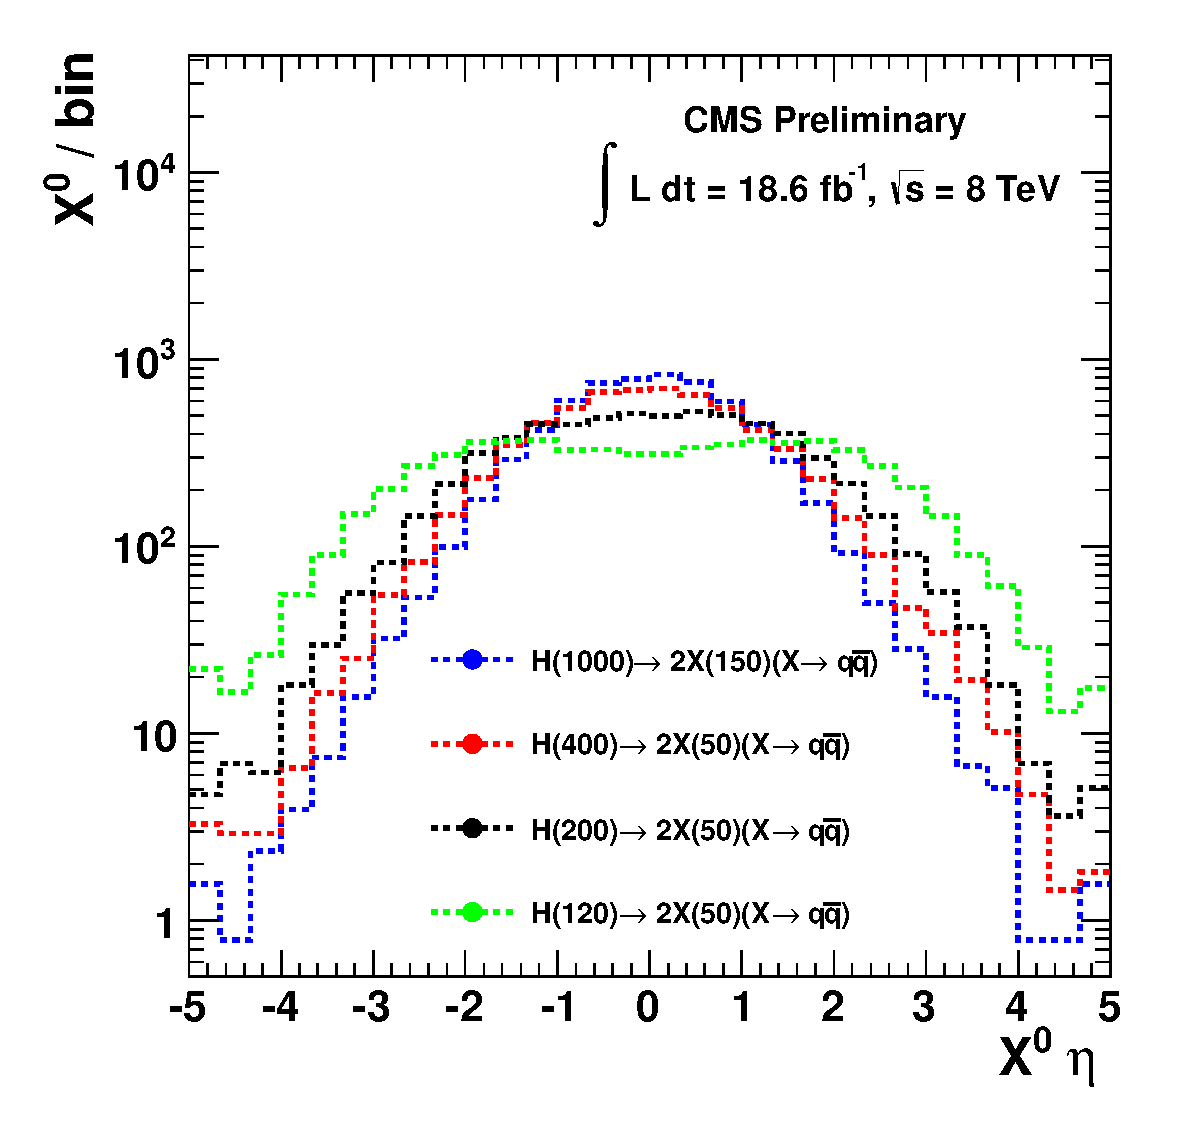
\includegraphics[width=0.495\textwidth]{plots/signal/xeta.pdf}
\caption{Generated \Higgs $p_T$ and \X $p_T$ and $\eta$ distributions for selected signal models.\label{fig:sigHX}}
\end{figure}

An example of a fully reconstructed
simulated signal event is presented in Figure \ref{fig:eventDisplay}.

\begin{figure}[htbp]
\centering
 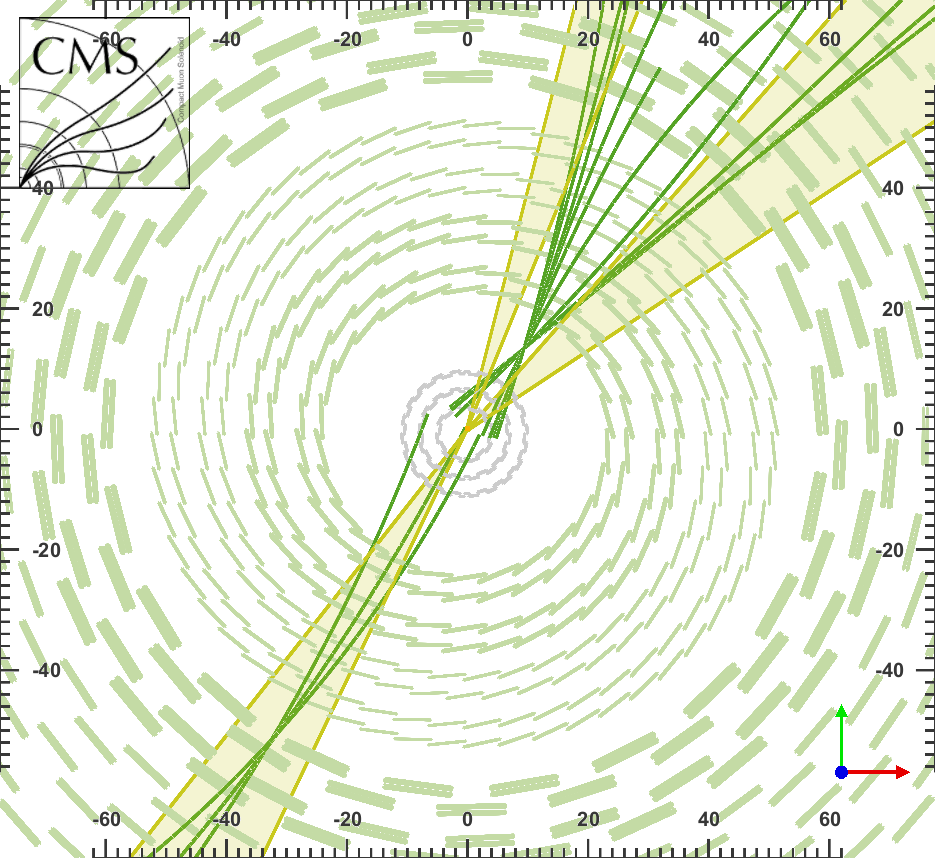
\includegraphics[width=0.8\textwidth]{plots/eventDisplay.png}
\caption{CMS event display of an example simulated signal event with a dijet pair originating from a transversly displaced secondary vertex.
The event is presented in a plane transverse to the LHC beam line.
The concentric layers of detectors (grey or light green) show the tracker detector modules, the
yellow cones correspond to reconstructed jets, while the thick green lines are charge particles
trajectories. A displaced secondary vertex is clearly visible with a dijet pair moving towards
top-right corner of the picture.
The axis labels use \cm units. \label{fig:eventDisplay}}
\end{figure}


The background of the search consists of events containing hadronic jets. Many Standard Model processes
produce multiple jets in the event, however, given the considered phase space and the SM production
cross sections,
 the most significant background 
is expected to arise from QCD events. The corresponding simulated samples
are listed in Table~\ref{tab:backgrMC}. The samples are binned in terms
of the transverse momentum transfer between the colliding partons, $\hat{p_T}$.
The resulting transverse sum
of the jets, $H_T$, for these events corresponds to approximately twice the value of $\hat{p_T}$. 
For each simulated background sample the number of events passing the signal trigger
scaled to the total integrated luminosity is shown. The per event weight factors that need 
to be applied in order to compare the simulated samples with the data are also given. These
arise simply from the cross section of the process, total integrated luminosity and the number
of events simulated for each dataset.
The weight factors for samples with $\hat{p_T}$
below 470\GeV are significantly above 1, therefore the amount of simulated events in this region is insufficient.
The background contribution
significantly decreases with increased $\hat{p_T}$, therefore we do not consider samples with $\hat{p_T}$ higher
than 800\GeV. For QCD events with $\hat{p_T}$ below 80\GeV the small efficiency of passing the trigger
 requirement of $H_T>$300\GeV
makes the low $\hat{p_T}$ contribution negligible.

\begin{table}[hbtp]
\begin{center}
\begin{tabular}{lccc}
\hline
 \multicolumn{1}{c}{Dataset name} & Cross section  & N events passing  & Per event \\
                                    &     (pb)       & the trigger / 18.6 \fbinv & weight factor \\
\hline
\texttt{\small QCD (600$<\hat{p_T}<$800\GeV)}               & 2.70e1       & 4.5e2 & 0.1  \\
\texttt{\small QCD (470$<\hat{p_T}<$600\GeV)}               & 1.14e2       & 1.7e3 & 0.6 \\
\texttt{\small QCD (300$<\hat{p_T}<$470\GeV)}               & 1.76e3        & 2.6e4 & 5.5 \\
\texttt{\small QCD (170$<\hat{p_T}<$300\GeV)}               & 3.41e4 & 5.2e5 & 1.1e2 \\
\texttt{\small QCD (120$<\hat{p_T}<$170\GeV)}               & 1.56e5  & 7.5e5 & 4.8e2 \\
\texttt{\small QCD (80$<\hat{p_T}<$120\GeV)}                & 1.03e6  & 4.8e5 & 3.2e3 \\
\texttt{\small QCD (50$<\hat{p_T}<$80\GeV)}                & 8.15e6  & 1.1e5 & 2.5e4 \\
\hline
\end{tabular}
\caption{Simulated background samples used in the analysis.\label{tab:backgrMC}}.
\end{center}
\end{table}
